\documentclass[10pt]{beamer}

\usetheme[progressbar=frametitle]{metropolis}
\usepackage{appendixnumberbeamer}
\usepackage{silence}
\WarningsOff*

\usepackage{booktabs}
\usepackage[scale=2]{ccicons}

\usepackage{pgfplots}
\usepgfplotslibrary{dateplot}

\usepackage{xspace}
%\newcommand{\themename}{\textbf{\textsc{metropolis}}\xspace}

\usepackage{graphicx}
\usepackage{multicol, multirow}
\usepackage{hyperref}
\usepackage{amsmath, amssymb, amsfonts}

\title{Onset Detection}
\subtitle{An interesting approach to Query by Humming systems}
\date{April 30, 2019}
\author{
Soham Bonnerjee (BS1609)\\
Subhrajyoty Roy (BS1613)\\
Ritwik Bhaduri (BS1616)}
\institute{B.Stat., Indian Statistical Insitute, Kolkata}
% \titlegraphic{\hfill\includegraphics[height=1.5cm]{logo.pdf}}

\begin{document}
\maketitle

\begin{frame}{Table of contents}
  \setbeamertemplate{section in toc}[sections numbered]
  \tableofcontents[hideallsubsections]
\end{frame}

% INTRODUCTION
\section{Introduction}

\begin{frame}[fragile]{Visions}
\begin{enumerate}
    \item \texttt{THE STORY:} Where you might need it?
    \pause
    \item \texttt{3 Stage Procedure:}
    \begin{enumerate}
        \item Building the database of songs.
        \item Detection of onsets (beats in layman's terms) of hummed song.
        \item Return the song which matches the most.
    \end{enumerate}
\end{enumerate}

\end{frame}

\begin{frame}{How is Digital Audio stored?}
    \begin{itemize}
        \item \texttt{Sampling:} The binning in $x$-axis. Generally $44100$ samples per second.
        \item \texttt{Quantization:} The binning in $y$-axis. Generally, ranges from $-(2^{15}-1)$ to $+(2^{15} -1)$ for $16$ bit machine.
    \end{itemize}
\end{frame}

\begin{frame}{How does Digital Audio look like? (Toy Example)}
    \begin{figure}
        \centering
        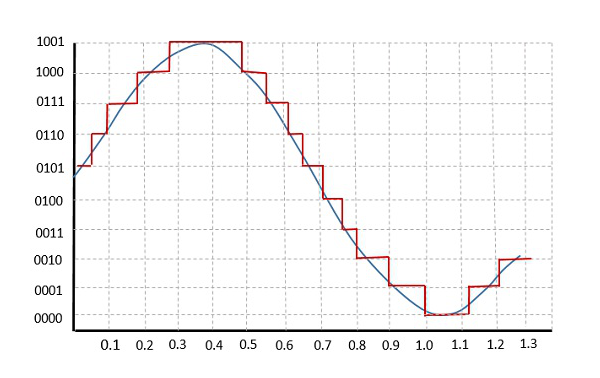
\includegraphics[width = \textwidth]{fig/quantization.jpg}
    \end{figure}
\end{frame}

\begin{frame}{How does Digital Audio look like? (Real Example)}
    \begin{figure}
        \centering
        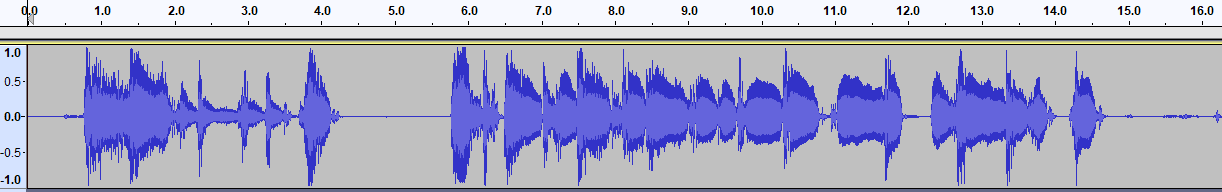
\includegraphics[width = \textwidth,trim={0 0 22cm 0},clip]{fig/oscillogram_sa_re_jahan_se_accha.png}
    \end{figure}
\end{frame}

\begin{frame}{What is Onset?}
    \begin{figure}
    \centering
    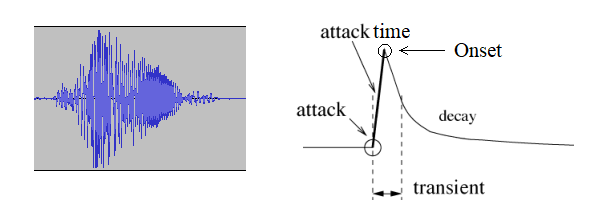
\includegraphics[width = \textwidth]{fig/onset_defn.png}
    \end{figure}
\end{frame}


\begin{frame}{Discrete Fourier Transform (DFT)}
    \begin{itemize}
        \item Let digital audio is denoted by a finite sequence or equivalently a vector of numbers, $\textbf{x} = x[0], x[1], \dots x[N-1]$, where $N$ is the number of samples taken in the whole audio.
        \item Define the inner product: $\langle \textbf{x},\textbf{y} \rangle = \sum_{k=0}^{N-1} x[k]\bar{y}[k]$
        \item The pure digital tones of order $N$ of frequency $f$ is the following complex $N$ length vector;
        $$v_{f} = \dfrac{1}{\sqrt{N}}\left(1, e^{2\pi i f/N}, e^{4\pi i f/N}, e^{6\pi i f/N}, \dots e^{2\pi i f(N-1)/N}\right)$$
        \item DFT of $\textbf{x}$ is $\textbf{y}$, where;
        $$y[k] = \langle \textbf{x}, v_k \rangle = \dfrac{1}{\sqrt{N}}\sum_{n=0}^{N-1} x[n] e^{-2\pi i fn/N}$$
        for $k = 0, 1, \dots (N-1)$.
    \end{itemize}
\end{frame}

\begin{frame}{Short Time DFT}
    The STDFT of a signal $\textbf{x}$ at a position $n$ is given by;
    $$X_k(n) = \sum_{m= -\omega/2}^{\omega/2}x[n+m]e^{-2\pi i km/\omega}$$
    where $\omega$ is the window length. This $X_k(n)$ is called Short Time Fourier coefficient of discrete frequency $k$ at position $n$, representing the frequency content of frequency $k/\omega\times S_f$ during $t_n$ to $t_{n+\omega}$.
\end{frame}

\section{Building the Database}
\begin{frame}{Database}
    \begin{enumerate}
        \item For our experiment, we use a database of 10 songs.
        \item For each song, the onsets are determined from the instrumental notations.
        \item A typical element of database is a vector of size $20$ to $35$, containing the onset times of first verse of the song.
    \end{enumerate}
\end{frame}

\begin{frame}{10 Chosen songs in Database}
    \begin{multicols}{2}
    \begin{enumerate}
        \item Jana Gana Mana.
        \item Ekla Cholo Re.
        \item Ore Grihobasi.
        \item Sa Re Jahan Se Accha.
        \item Esho Shyamolo Shundoro.
        \item Jingle Bells.
        \item My Heart will go on.
        \item Fur Elise.
        \item Hain Apna Dil.
        \item Jindegi Ek Safar.
    \end{enumerate}
    \end{multicols}
\end{frame}

\begin{frame}{How the vector of onsets are created?}
    For example, consider \textit{sargam} of \textit{Ekla Cholo Re}
    $$\vert Na Na Na \vert Sa - Sa \vert Re Re - \vert Pa - - \vert Ma - - \vert Ga - - \vert Re Sa - \vert Re Ga Ga \vert Re Sa - \vert$$
    gets converted to the vector;
    $$\vert 1, 2, 3, \vert 4, 6, \vert 7, 8, \vert 10,\vert 13, \vert 16,\vert 19, 20, \vert 22, 23, 24, \vert 25, 26,\vert$$
\end{frame}


\section{Onset Detection Methods}

\begin{frame}{3 Stage Procedure}
    \begin{enumerate}
    \item \textbf{Preprocessing:} It allows the raw vector of signal to be transformed slightly in order to improve the performance of the subsequent analysis. This step is optional and highly depends on the type of signal you are analyzing.
    \pause
    \item \textbf{Detection Function:} A detection function is a statistic which sufficiently reduce the data in a more compact form keeping the necessary information about the presence or the strength of the signal in a local neighbourhood. A detection function is applied to the signal through a sliding window (or moving window), allowing only the neighbourhood signal to be summarized.
\end{enumerate}

\end{frame}

\begin{frame}{3 Stage Procedure (Contd.)}
    \begin{enumerate}
        \item For example, let $\omega$ is the size of the sliding window, and let $T(\cdot)$ be the statistic to be applied. Then, this detection function computes the value of the statistic for each of the moving window;
        $$T[n] = T(x[n], x[n+1], \dots x[n+\omega - 1]) \qquad \forall n = 0,1,2, \dots (N-\omega)$$
        The statistic $T(\cdot)$ is chosen in a way so that the onset at time $t_n$ results in a comparatively higher value of $T[n]$ rather than its other values.
        \pause
        \item \textbf{Peak Detection:} The resulting detection function is desired to produce local maximums at the time of the true onsets. Therefore, a peak detection algorithm is run at the end to identify the peaks in the vector of detection function. The times corresponding to these peaks are finally identified as possible onsets.
    \end{enumerate}
\end{frame}

\begin{frame}{Energy Detector}
We consider the detection of presence of a signal in the $n^\text{th}$ time-point.
\begin{align*}
H_0: x[n]=w[n]  &&  n=0,1,\cdots, \omega-1\\ 
H_1: x[n]=s[n]+w[n] && n=0,1,\cdots, \omega-1 
\end{align*}
where $s[n]$ is deterministic and \textit{completely unknown}, and $w[n]$ is WGN (White Gaussian Noise) with variance $\sigma^2$.
\end{frame}

\begin{frame}{Energy Detector (Contd.)}
    Using Likelihood ratio test, we reject $H_0$ in favour of $H_1$ if
\begin{align}
   T(\textbf{x})= \displaystyle\sum_{n=0}^{\omega-1}x^2[n] > \gamma'
\end{align}
This detector computes the \textit{local energy} in the received data and compares it to a threshold. Hence this statistic is known as \textit{Energy Detector}.
\end{frame}


\begin{frame}{Problem with Energy Detector}
    Energy Detector is unable to detect immediate changes in local energy. Hence, unable to detect onsets if \textit{Meends}\footnote{Meends are sliding from one note to another} are present.
    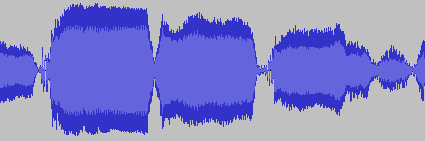
\includegraphics[width = \textwidth]{fig/onset_blob.png}
\end{frame}


\begin{frame}{Spectral Dissimilarity}
    $$T(n) = \sum_{k} \left(\vert X_k(n) \vert - \vert X_k(n-1) \vert\right) \textbf{1}_{\left\{\vert X_k(n) \vert > \vert X_k(n-1) \vert\right\}}$$
    \begin{enumerate}
        \item Detect immediate changes in whole range of frequency spectrum.
        \item Focus on onsets rather than offsets.
    \end{enumerate}
\end{frame}

\begin{frame}{Dominant Spectral Dissimilarity}
    \begin{align*}
H_0: x[n]&=w[n] && n=0,1,\cdots, \omega-1\\\\ 
H_1: x[n]&= \smash{\left\{\begin{array}{@{}l@{}}
           w[n] \\[\jot] 
           A\cos(2\pi f_0n+\phi)+w[n] \\[\jot] 
           \end{array}\right.} && n=0,\cdots, n_0-1, n_0+M, \cdots, \omega-1 \\
  & && n=n_0,n_0+1,\cdots, n_0+M-1
 \end{align*}
where $w[n]$ is WGN with known variance $\sigma^2$, and $A$, $f_0$, $\phi$ are \textit{Amplitude}, \textit{Frequency}, and \textit{Phase} respectively. These parameters might be unknown.
\end{frame}

\begin{frame}{Dominant Spectral Dissimilarity (Contd.)}
    Likelihood Ratio test reject $H_0$ in favour of $H_1$ if;
    $$T(x) = \dfrac{4}{\omega}\max_{f_0}\dfrac{1}{\omega}\left|\displaystyle\sum_{n=0}^{\omega-1}x[n]\exp(-i2\pi f_0n)\right|^2 > \gamma$$
    equivalently, if the maximum of the magnitudes of the DFT frequency contents is large enough.\\
    Combining this, and idea of detecting instantaneous changes;
    $$T[n] = \left(\max_k \vert X_k(n)\vert^2 - \max_k\vert X_k(n-1)\vert^2\right)\times \textbf{1}_{\left\{\max_k \vert X_k(n)\vert > \max_k\vert X_k(n-1)\vert\right\}}$$
\end{frame}


\begin{frame}{Peak Detection: Features of a peak}
    \begin{enumerate}
    \item Due to randomness in noise, it might happen that the detection function shows a peak at a location where there is only noise. Such peaks would be of relatively smaller height than a peak where onset has occurred. Therefore, we must choose a threshold parameter so that the peaks below that threshold parameter is completely ignored.
    \item A peak should be of a higher value that its neighbouring values of detection function. Therefore, we must compare its value of detection function with that of its predetermined neighbours.
    \item Two peaks should not be too close to each other. Two consecutive sounds must be at least $1/10$-th of a second apart in time to be heard as distinguished sounds. Therefore, a reasonable peak detection algorithm should merge two onsets into a single one if they are less than 0.1 second apart.
\end{enumerate}
\end{frame}

\section{Power Calculation}
\begin{frame}{Basic Power Calculation}
    \begin{align*}
 x[k] & \sim N(0, \sigma^2) &&  k=0,1,\cdots, k^*-1\\ 
 x[k] & \sim N\left(Ae^{-\lambda\dfrac{k-k^*}{S_f}}\cos{\left(2\pi f_0\dfrac{k-k^*}{S_f}\right)}, \sigma^2\right) && k=k^*,k^* + 1,\cdots, N-1 
 \end{align*}

\end{frame}


\begin{frame}{Two main Results}

\texttt{\textbf{Result 1}}
\begin{align*}
    & P\left(\hat{k}\text{ is an outputted onset}\right)\\
\geq & \min\left\{0, \sum_{n=(-r)}^{r}P(T[\hat{k}] > T[\hat{k} + nh]) + P(T[\hat{k}] > \alpha) - 2r\right\}
\end{align*}
Helps to say with confidence, a true onset is detected.\\
\vspace*{1cm}

\texttt{\textbf{Result 2}}
$$P\left(\hat{k}\text{ is an outputted onset}\right) < \frac{1}{2}\left( P(T[\hat{k}]>\alpha) (2 - P(T[\hat{k}] > \alpha)) \right)$$
when $k$ is at least $\omega$ samples away from $k^*$. Helps to bound false positive probability.
\end{frame}

% say about the chi-square distribution of energy detector and distribution of fourier spectrum


\begin{frame}{Power of Energy Detector}
    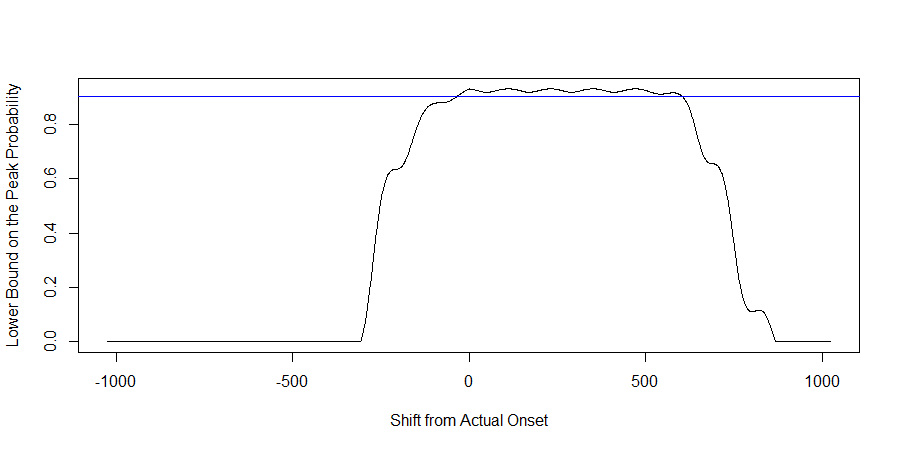
\includegraphics[width=\textwidth]{fig/power_energy.png}
\end{frame}

\begin{frame}{Power of Spectral Dissimilarity}
    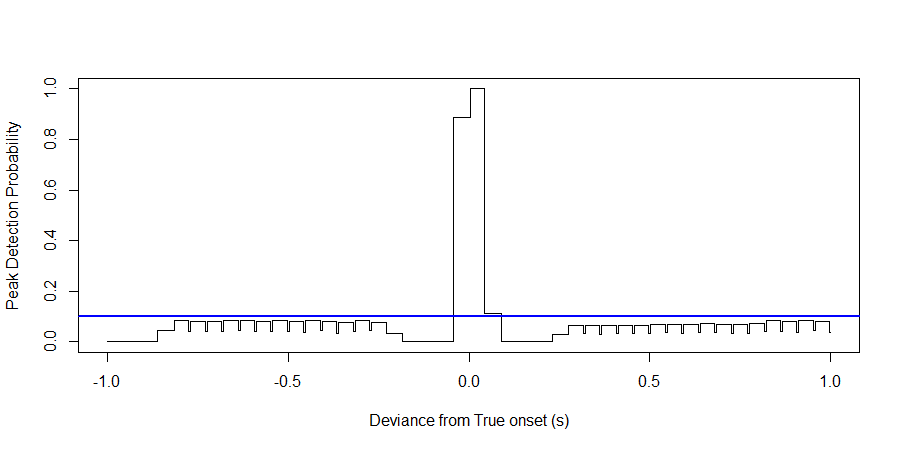
\includegraphics[width=\textwidth]{fig/power_spectral.png}\\
    Blue line is $y = 0.1$.
\end{frame}

\begin{frame}{Power of Dominant SD}
    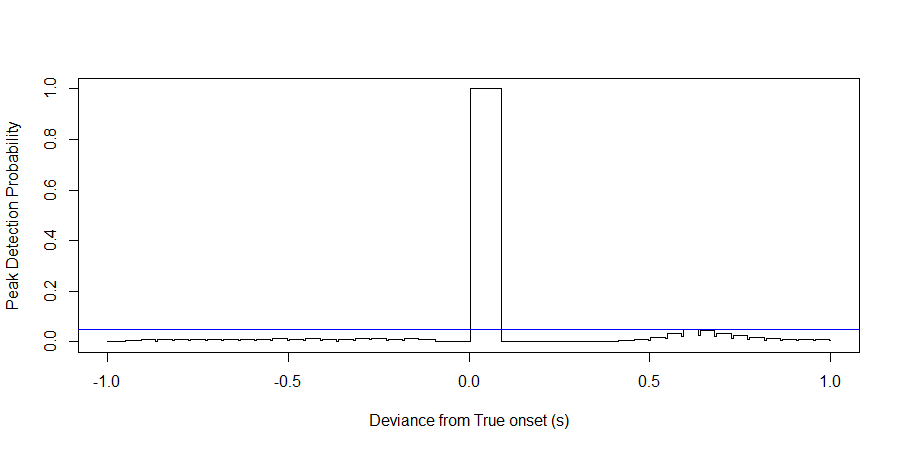
\includegraphics[width=\textwidth]{fig/power_dfreq.png}\\
    Blue line is $y = 0.05$.
\end{frame}

\section{Searching the database}

\begin{frame}{Subset Matching}
\texttt{Assumption:} Both the songs are assumed to be in the same unit with respect to time. It means that the same verse is present in both the songs and the time taken to sing both the parts is equal.

\begin{figure}
    \centering
    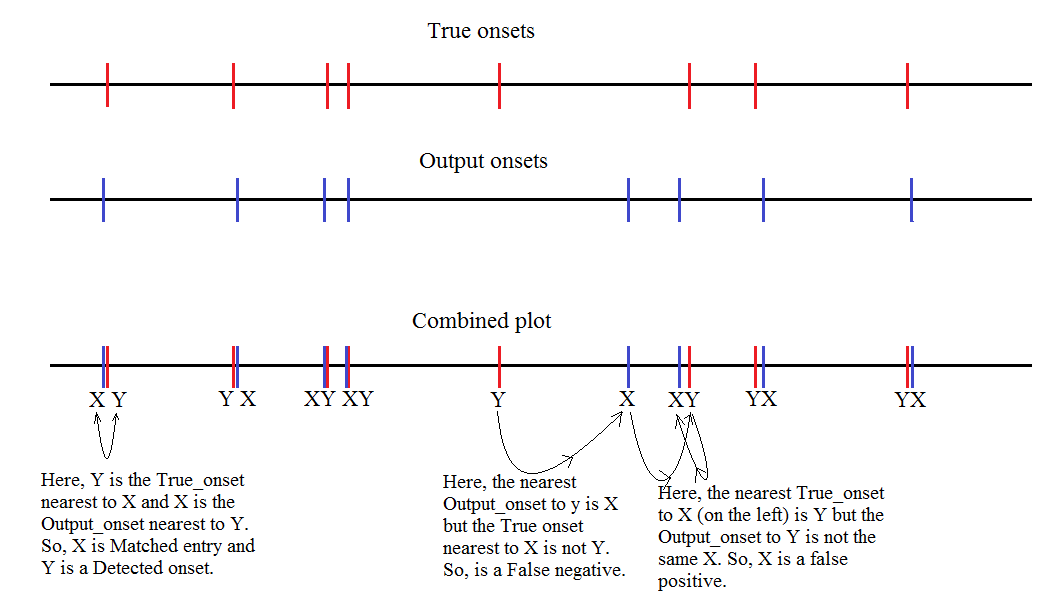
\includegraphics[width = \textwidth]{fig/subset_matching.png}
\end{figure}
\end{frame}

\begin{frame}{Correlative Matching}
    \begin{enumerate}
        \item \texttt{Assumption:} First and last true onsets are detected.
        \item Find all possible matches of First and last true onsets.
        \item For each matchings, compute the linear transformation.
        \item Perform subset matching on transformed onsets.
        \item Compute score for each transformation:
        \begin{align*}
            Score & = Cor(matched\_output, matched\_transformed\_true\_onset)\\
            & \times \left(1 - \dfrac{\#False\_positive}{output\_length}\right) \times \left(1 - \dfrac{\#False\_negative}{true\_onset\_length}\right)
        \end{align*}
    \end{enumerate}
\end{frame}

\section{Experimental Results}

\begin{frame}{Basic Setup}
    \begin{enumerate}
        \item 3 hummed song. 
        \begin{enumerate}
            \item \textit{Sa Re Jahan Se Accha}; for finding the optimal hyperparameter tuning.
            \item \textit{Ekla Cholo Re}; to study effect of meends.
            \item \textit{Jingle Bells}; to study effect of changing pitches.
        \end{enumerate}
        \item 10 songs in database.
    \end{enumerate}
\end{frame}

\begin{frame}{Optimal Hyperparameter Setup}
    \begin{enumerate}
        \item  Local Energy Detector, window length of 4096 samples, hopsize of 512 samples. For peak
        detection procedure, it computes a peak with its 8 neighbouring points to both sides, and use a mean based
        thresholding criterion.
        \item  Spectral Dissimilarity Detector, window length of 4096 samples, hopsize of 2048 samples. For peak detection procedure, it computes a peak with its 4 neighbouring points to both sides, and use a mean based thresholding criterion.
        \item Dominant Spectral Dissimilarity Detector, window length of 4096 samples, hopsize of 2048 samples. For peak detection procedure, it computes a peak with its 2 neighbouring points to both sides, and use a mean based thresholding criterion.
    \end{enumerate}    
\end{frame}

\subsection{First Song}
{\setbeamercolor{palette primary}{fg=white, bg=gray}
\begin{frame}[standout]
  \texttt{Song 1: Sa Re Jahan Se Accha}
\end{frame}
}

\begin{frame}{Performance of Local Energy Detector}
    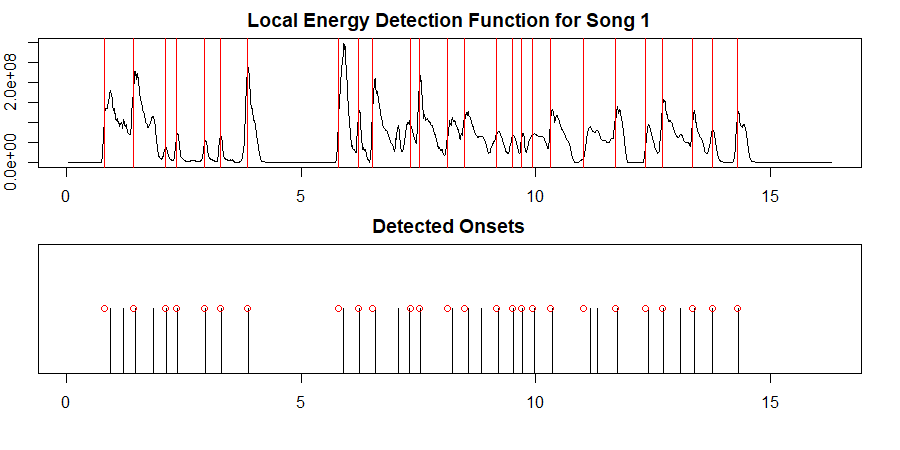
\includegraphics[width = \textwidth]{fig/energy_song1.png}
\end{frame}

\begin{frame}{Performance of Spectral Dissimilarity}
    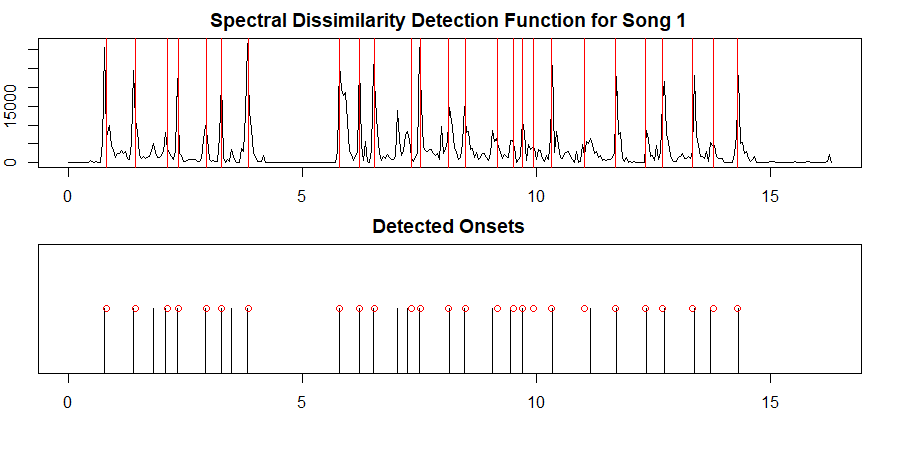
\includegraphics[width = \textwidth]{fig/spectral_song1.png}
\end{frame}

\begin{frame}{Performance of Dominant Spectral Dissimilarity}
    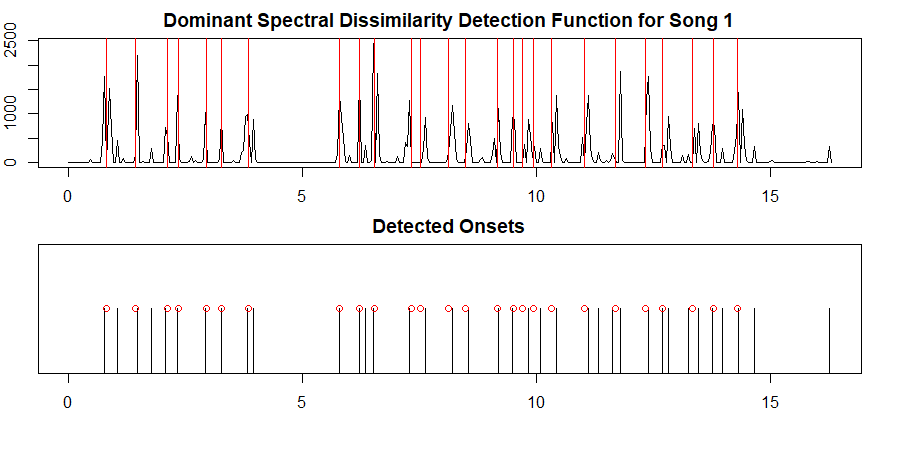
\includegraphics[width = \textwidth]{fig/dfreq_song1.png}
\end{frame}

\begin{frame}{Performance of Searching Algorithm}
\begin{table}
\centering
\caption{Details of Searching Output using hummed version of \textit{Sa Re Jahan Se Accha}}
\resizebox{\textwidth}{!}{
\begin{tabular}{|c|c|c|c|c|c|c|}
\hline
\multirow{2}{*}{Ranks} & \multicolumn{2}{c|}{Energy Detector} & \multicolumn{2}{c|}{Spectral Dissimilarity} & \multicolumn{2}{c|}{Dominant SD} \\ \cline{2-7} 
                       & Song                     & Score     & Song                         & Score        & Song                   & Score   \\ \hline
1                      & Sa Re Jahan Se Accha     & 0.75      & Sa Re Jahan Se Accha         & 0.791        & Sa Re Jahan Se Accha   & 0.649   \\ \hline
2                      & Jingle Bells             & 0.573     & Jingle Bells                 & 0.595        & Fur Elise              & 0.623   \\ \hline
3                      & Jana Gana Mana           & 0.568     & Jana Gana Mana               & 0.585        & Jingle Bells           & 0.544   \\ \hline
4                      & Hain Apna Dil            & 0.53      & Jindegi Ek Safar             & 0.578        & Jana Gana Mana         & 0.541   \\ \hline
5                      & Jindegi Ek Safar         & 0.506     & My Heart will go on          & 0.578        & Ore Grihobasi          & 0.493   \\ \hline
\end{tabular}
}
\end{table}
\end{frame}

\subsection{Second Song}
{\setbeamercolor{palette primary}{fg=white, bg=gray}
\begin{frame}[standout]
  \texttt{Song 2: Ekla Cholo Re}
\end{frame}
}

\begin{frame}{Performance of Local Energy Detector}
    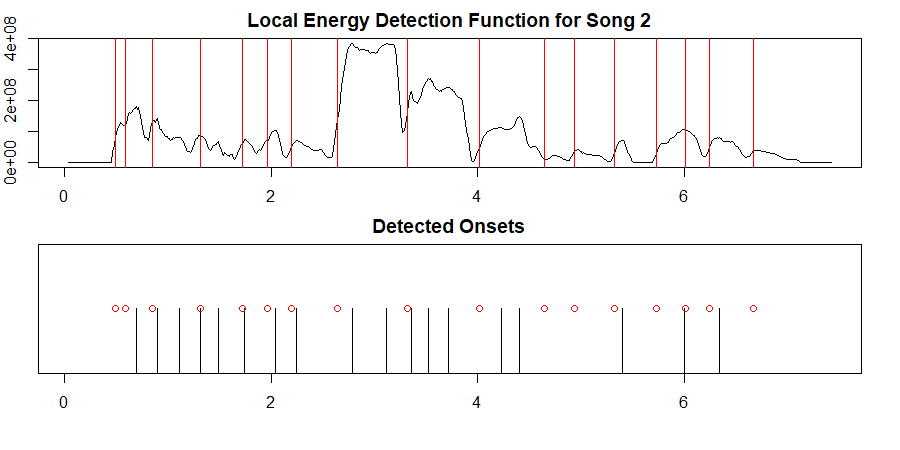
\includegraphics[width = \textwidth]{fig/energy_song2.png}
\end{frame}

\begin{frame}{Performance of Spectral Dissimilarity}
    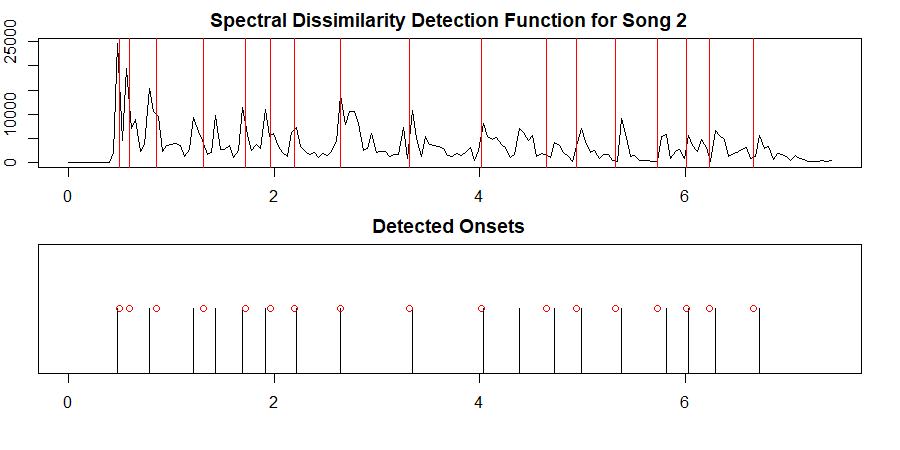
\includegraphics[width = \textwidth]{fig/spectral_song2.png}
\end{frame}

\begin{frame}{Performance of Dominant Spectral Dissimilarity}
    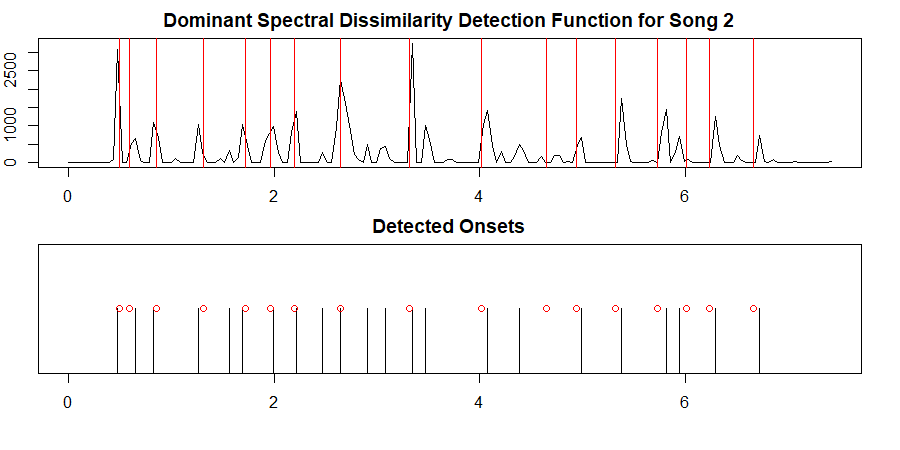
\includegraphics[width = \textwidth]{fig/dfreq_song2.png}
\end{frame}

\begin{frame}{Performance of Searching Algorithm}

\begin{table}
\centering
\caption{Details of Searching Output using hummed version of \textit{Ekla Cholo Re}}
\resizebox{\textwidth}{!}{
\begin{tabular}{|c|c|c|c|c|c|c|}
\hline
\multirow{2}{*}{Ranks} & \multicolumn{2}{c|}{Energy Detector} & \multicolumn{2}{c|}{Spectral Dissimilarity} & \multicolumn{2}{c|}{Dominant SD} \\ \cline{2-7} 
                       & Song                  & Score        & Song                      & Score           & Song                   & Score     \\ \hline
1                      & Ekla Cholo Re         & 0.64         & Ekla Cholo Re             & 0.735           & Ekla Cholo Re          & 0.684     \\ \hline
2                      & Hain Apna Dil         & 0.552        & Hain Apna Dil             & 0.551           & Jana Gana Mana         & 0.668     \\ \hline
3                      & Jana Gana Mana        & 0.522        & Jana Gana Mana            & 0.509           & My Heart will go on    & 0.657     \\ \hline
\end{tabular}
}
\end{table}
\end{frame}

\subsection{Third Song}
{\setbeamercolor{palette primary}{fg=white, bg=gray}
\begin{frame}[standout]
  \texttt{Song 3: Jingle Bells}
\end{frame}
}

\begin{frame}{Performance of Local Energy Detector}
    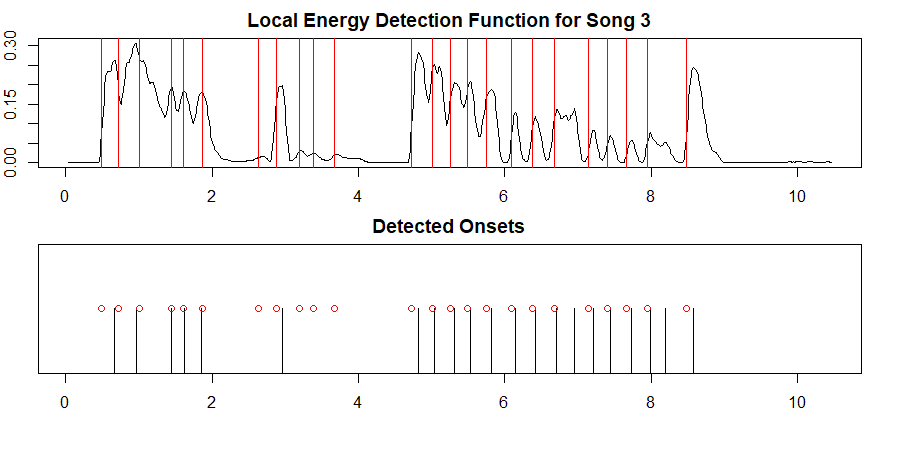
\includegraphics[width = \textwidth]{fig/energy_song3.png}
\end{frame}

\begin{frame}{Performance of Spectral Dissimilarity}
    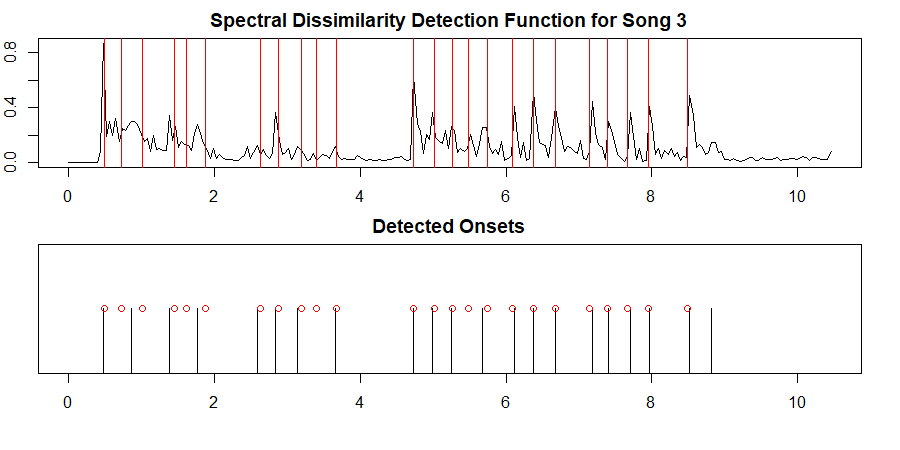
\includegraphics[width = \textwidth]{fig/spectral_song3.png}
\end{frame}

\begin{frame}{Performance of Dominant Spectral Dissimilarity}
    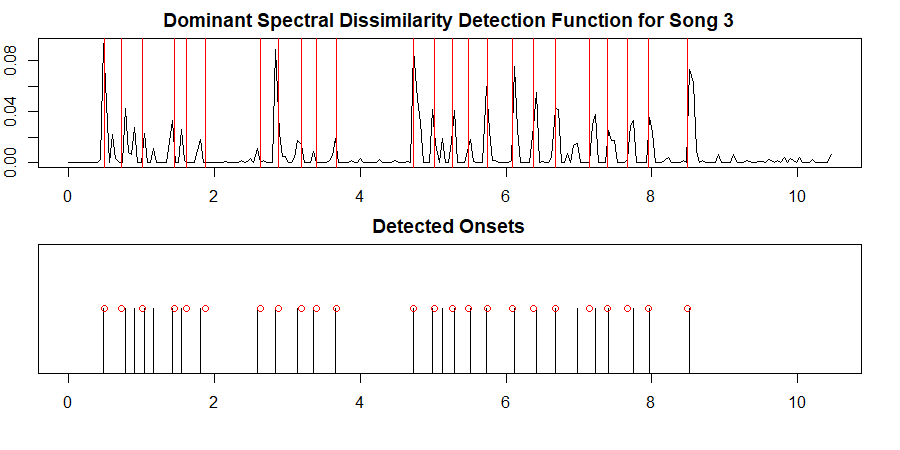
\includegraphics[width = \textwidth]{fig/dfreq_song3.png}
\end{frame}

\begin{frame}{Performance of Searching Algorithm}

\begin{table}
\centering
\caption{Details of Searching Output using hummed version of \textit{Jingle Bells}}
\resizebox{\textwidth}{!}{
\begin{tabular}{|c|c|c|c|c|c|c|}
\hline
\multirow{2}{*}{Ranks} & \multicolumn{2}{c|}{Energy Detector} & \multicolumn{2}{c|}{Spectral Dissimilarity} & \multicolumn{2}{c|}{Dominant SD} \\ \cline{2-7} 
    & Song                  & Score        & Song                      & Score           & Song                   & Score     \\ \hline
1   & Jindegi Ek Safar  & 0.608  & Hain Apna Dil & 0.716  &  Jingle Bells    & 0.72     \\ \hline
2       & Hain Apna Dil         & 0.549        & Jindegi Ek Safar             & 0.716           & Jindegi Ek Safar         & 0.644     \\ \hline
3   &   Ekla Cholo Re     & 0.548        & Jingle Bells   & 0.687           & Hain Apna Dil   & 0.607  \\ \hline
\end{tabular}
}
\end{table}
\end{frame}

\section{Conclusion}

\begin{frame}{Summary}
\begin{enumerate}
    \item Local Energy detector does not perform well under different note variants (or Alankars, e.g. Meend).
    \item Spectral Dissimilarity detection suffers from the changes in the noise pattern and in pitches.
    \item Dominant Spectral Dissimilarity is better than the previous two approaches, as it does not skip a true onset. Although, it suffers from the detection of more false positives than other approaches, the system as a whole works better with this.
\end{enumerate}
\end{frame}

\begin{frame}{Advantages over other QBH system}
    \begin{enumerate}
    \item Most of the typical methods for QBH use the pitch information in the hummed song. Our method relies more on the rhythm of the song. So when some input is somewhat inharmonious or off-key most of the traditional systems fail but our method performs rather well.
    \item Our method compares the onsets of the hummed song with that of the songs in the database. This eliminates the need of storing the entire songs in the database. We just need to store the onsets of the song in the database. This results in a huge reduction in the storage space.
    \item Most QBH systems require a song to be sung by a handful of singers so that the algorithm can compare the hummed song with the different versions of the same song. This entails a lot of human effort to generate the database. Our approach doesn't require any human singing but the onsets of the actual song which is accessible from online sources.
\end{enumerate}
\end{frame}

\begin{frame}{Future Scopes}
    \begin{enumerate}
    \item We perform the analysis assuming the fact that the noise are independent and identically distributed according to normal distribution with mean $0$ and constant variance $\sigma^2$. However, in practice, this assumption might not be true, as there might be different correlation structure between these errors.
    \item It would be better if some tighter bounds on the probability of type I error and type II errors are available for the three detection algorithms.
    \item Usage of dynamic time wraping method rather than simple correlation to improve the searching technique.
    \item Our algorithm demands the user to sing the first verse of the song. However, the point where the first verse ends may not be known to the user. In such case, searching procedure also should be able to match prefix of the song.
\end{enumerate}

\end{frame}


\appendix

\begin{frame}[allowframebreaks]{References}
\begin{thebibliography}{9}
\bibitem{statsignal} 
Steven M. Kay, \textit{Fundamentals of Statistical Signal Processing, Volume II: Detection Theory}. Prentice-Hall, 1998.

\bibitem{bello.et.al}
J. P. Bello, L. Daudet, S. Abdallah, C. Duxbury, M. Davies and M. B. Sandler, \textit{A tutorial on onset detection in music signals}, in IEEE Transactions on Speech and Audio Processing, vol. 13, no. 5, pp. 1035-1047, Sept. 2005.

\bibitem{kauppinen}
I. Kauppinen, \textit{Methods for detecting impulsive noise in speech and audio signals}, 2002 14th International Conference on Digital Signal Processing Proceedings. DSP 2002 (Cat. No.02TH8628), Santorini, Greece, 2002, pp. 967-970 vol.2.

\bibitem{holzapfel}
A. Holzapfel, Y. Stylianou, A. C. Gedik and B. Bozkurt, \textit{Three Dimensions of Pitched Instrument Onset Detection}, in IEEE Transactions on Audio, Speech, and Language Processing, vol. 18, no. 6, pp. 1517-1527, Aug. 2010.

\bibitem{fourier}
Uniservity of Oslo: Sound Processing Lecture Part I: \textit{Fourier analysis and applications to sound processing}. \url{https://www.uio.no/studier/emner/matnat/math/nedlagte-emner/MAT-INF2360/v12/part1.pdf}.

\bibitem{complex}
Amos Lapidoth. \textit{A Foundation in Digital Communication} ETH Zurich. Swiss Federal Institute of Technology. 2009.
\end{thebibliography}
\bibliographystyle{abbrv}
\end{frame}


{\setbeamercolor{palette primary}{fg=black, bg=white}
\begin{frame}
  \centering
  \Huge{\texttt{\textbf{THANK YOU}}}
\end{frame}
}


{\setbeamercolor{palette primary}{fg=black, bg=yellow}
\begin{frame}[standout]
  \Huge
  \textsc{Questions?}
\end{frame}
}



\end{document}
